\documentclass[11pt]{article}
  
%%% LATEX COMMON Packages 

\usepackage[bookmarks,colorlinks,breaklinks]{hyperref}  % PDF hyperlinks, with coloured links
\hypersetup{linkcolor=blue,citecolor=blue,filecolor=blue,urlcolor=blue} % all blue links
\usepackage{amsmath,amsfonts,amsthm,amssymb,environ,xstring}
\usepackage{dsfont}
\usepackage{fullpage}
\usepackage{mdframed}
\usepackage{tikz}
\usepackage{graphicx}
\newcommand{\ignore}[1]{}


\title{\bf{CS 181: Homework 2}}
\author{ Einar Balan}
\date{}
\begin{document}
\maketitle
\begin{mdframed}
\textsc{Guidelines}:
\begin{itemize}
\item Upload your assignments to Gradescope by 9:59 PM. 
\item Follow the instructions mentioned on the course webpage for uploading to Gradescope very carefully (including starting each problem on a new page and matching the pages with the assignments); this makes it easy and smooth for everyone. As the guidelines are simple enough, bad uploads will not be graded. 
\item You may use results proved in class without proofs as long as you state them clearly.
\item Most importantly, make sure you adhere to the policies for academic honesty set out on the course \href{https://hackmd.io/@raghum/introtcs}{webpage}. The policies will be enforced strictly. Homework is a stepping stone for exams; keep in mind that reasonable partial credit will be awarded and trying the problems will help you a lot for the exams.
\item All problem numbers correspond to our text 'Introduction to Theory of Computation' by Boaz Barak. So, exercise a.b refers to Chapter a, exercise b.
\end{itemize}
\end{mdframed}



\begin{enumerate}
\item Exercise 5.4. You can assume that $m \leq 2^n$ for the problem. [1 point]

[Hint: We already had an upper bound on the number of circuits of size s in class (this also applied to multi-output functions so you can use that as is). Next, what is the total number of functions $f:\{0,1\}^n \rightarrow \{0,1\}^m$? To get an upper bound use the reasoning we used in class: Think of the large truth table containing the outputs for every possible input string and the number of ways to fill the table. (How many options per cell and how many cells?)

Now compare the number of circuits to the number of m-bit output functions as we did in class. You don't have to redo the arithmetic calculations we did in class - you can use those simplifications as is.]

\item Answer the following for the DFA shown in the figure [.75 point]:\\
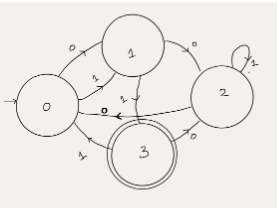
\includegraphics[width=2in]{DFA}

\begin{enumerate}
\item What is the set of accept states?
\item What sequence of states does the machine go through on input $1010101$?
\item Write down an accepting input for the machine.
\end{enumerate}

\item Draw a DFA that accepts strings which contain $011$ as a substring. For instance, $001100$, $00110$, $00000110111$ would be accepted whereas $010100$ should not be. [1 point]

[Hint: Think along the following lines: As you go over the input, you should initially skip all 1's. If you see a 0, then you may be onto something - it could be the first 0 of your sequence. If you see a 0 now, you can 'reset'. If you see a 1, you know you've seen a 0 and a 1. What should you look for next? You don't have to prove that you are correct - just the diagram with some explanations to make the grading easier would be enough.]

\item Use the construction we did in class to build a NFA for the Kleene star operation to build a NFA that accepts the strings $(\{01, 001\})^*$. [.75 point]

[Hint: Start with a DFA that only accepts $\{01, 001\}$ and then use the construction in class. You don't have to prove your construction works - just a diagram is enough (with some verbal explanations for clarity).]

\item For a language $L$, define $DROPLAST(L)$ to be the language containing all strings that can be obtained by removing the last symbol of a string in $L$. Thus, $DROPLAST(L) = \{x: xb \in L, \text{ for some }b \in \{0,1\}\}$. Show that if $L$ is computable by a DFA, then DROPLAST(L) is computable by a NFA. [.5 points]

[Hint: Think of adding appropriate $\varepsilon$ transitions to accepting states. You don't have to prove your construction works - just a diagram is enough (with some verbal explanations for clarity).]

\end{enumerate}

\end{document}

\item For a language $L$, define $DROPOUT(L)$ to be the language containing all strings that can be obtained by removing one symbol from a string in $L$. Thus, $DROPOUT(L) = \{a c : abc \in L, a, c \in \{0,1\}^*, b \in \{0,1\}\}$. Show that the class of regular languages is closed under DROPOUT. That is if $L$ is regular, then so is $DROPOUT(L)$. [1 point]

[Hint: Try to desgin a NFA for DROPOUT(L). To do so try to guess `where' the drop occurs, and use the idea from part(a). One idea is have two copies of the DFA for $L$, and then connect them based on a `guess' for where the drop is. So for example, think about how you would recognize a string obtained from L by dropping the second symbol. ]

